
\subsection{$\mathfrak{B}$-sheaf}
$\mathfrak{B}$-sheafはアフィンスキームの構成にも必要な概念で,ラフに言えばすべての開集合$U$に対して$\mathcal{F}(U)$が定まっているものではなく,
開基$\mathfrak{B}$の元$U$に対してだけ定まっている層を$\mathfrak{B}$-sheafという.

\Definition{
  位相空間$X$の\textbf{開基$\mathfrak{B}$が有限交叉で閉じている}とは,任意の$U,V\in \mathfrak{B}$に対して$U\cap V \in \mathfrak{B}$が成り立つことをいう. 
}

\Example{
  環$A$の素イデアルの集合$\spec{A}$の基本開集合による開基$\{D(f)\}_{f\in A}$は有限交叉で閉じている.
}{}

\Definition{
  $X$を位相空間.$\mathfrak{B}$をその開基とする.このとき$\mathcal{F}$が
  \textbf{$\mathfrak{B}$-前層($\mathfrak{B}$-presheaf)}であるとは,
  \begin{itemize}
    \item[---] $U\in \mathcal{B}$に対して$\mathcal{F}(U)$はアーベル群.
    \item[---] $V\subset U \in \mathcal{B}$に対して群準同型$\rho_{U,V}:\mathcal{F}(U) \to \mathcal{F}(V)$が定まる.
  \end{itemize}
  で,
  \begin{itemize}
    \item[(1)] $\rho_{U,U} = \text{id}_{\mathcal{F}(U)}$
    \item[(2)] 任意の開集合$W\subset V \subset U$に対して$\rho_{U,W} = \rho_{V,W}\circ \rho_{U,V}$となる.
  \end{itemize}
  を満たすときをいう.
}

\Definition{
  $\mathfrak{B}$が有限交叉で閉じているとする.このとき$\mathfrak{B}$-前層が層の条件を満たすとき
  \textbf{$\mathfrak{B}$-層($\mathfrak{B}$-sheaf)}という.
}

\Proposition{
  $\mathcal{F}$を$\mathfrak{B}$-前層とする.このとき,任意の開集合$V$に対して
  \begin{align*}
    \mathcal{F}(V)
      & = \varprojlim_{\substack{U\in \mathcal{B}                  \\ U\subset V}}\mathcal{F}(U)\\
      & = \left\{(s_{U})_{U} \in \prod_{\substack{U\in \mathcal{B} \\ U \subset V}} \mathcal{F}(U) \ \biggl|\
    \forall U' \subset U \in \mathcal{B}, s_{U}|_{U'}=s_{U'} \right\}
  \end{align*}
  制限写像は射影極限から誘導される射である.
  \begin{center}
    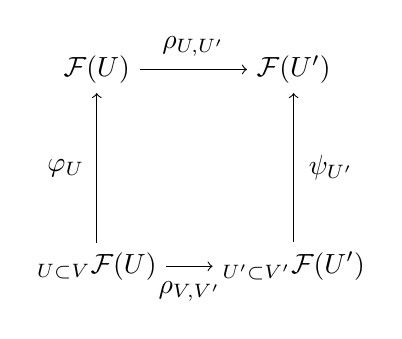
\begin{tikzpicture}[auto]
      \node (X1) at (0,0) {$\mathcal{F}(U)$};
      \node (X2) at (0,-2.5) {$\displaystyle \varprojlim_{U\subset V}\mathcal{F}(U)$};
      \node (Y1) at (2.5,0) {$\mathcal{F}(U')$};
      \node (Y2) at (2.5,-2.5) {$\displaystyle \varprojlim_{U'\subset V'}\mathcal{F}(U')$};
      \node (ci) at (1.25,-1.25) {$\circlearrowleft$};
  
      \draw[->] (X1) to node[yshift = -6pt,label=above:$\rho_{U,U'}$] () {} (Y1);
      \draw[->] (X2) to node[xshift = 6pt, label=left:$\varphi_{U}$] () {} (X1);
      \draw[->] (X2) to node[yshift = -2pt,label=below:$\rho_{V,V'}$] () {} (Y2);
      \draw[->] (Y2) to node[xshift = 2pt,label=right:$\psi_{U'}$] () {} (Y1);
    \end{tikzpicture}
  \end{center}
  するとこれは前層になる.
}{}

\Proposition{
  更に,$\mathfrak{B}$が有限交叉で閉じているなら,層になる.
}{
  任意の開集合$V$に対してその開被覆$\{V_{i}\}_{i}$を取る.ただし$V_{i} \in \mathfrak{B}$とする.\\
  \Claim{ (4)(Uniqueness)が成立する}\\
  $s\in \mathcal{F}(V)$が任意の$i$に対して$s|_{V_{i}} = 0$とする.今定義から$s=0$とは
  $U\subset V$なる任意の$U\in \mathfrak{B}$に対して$s_{U}\in \mathcal{F}(U)$が$0$であること
  である.実際$V$の開被覆から$U$の開被覆$\{U\cap V_{i}\}_{i} \subset \mathfrak{B}$を得る.
  また任意の$i$に対して$U\cap V_{i} \subset V_{i}$より$s|_{V_{i}}|_{U\cap V_{i}} = s|_{U\cap V_{i}} = 0$となる.従って任意の$i$に対して$s_{U}|_{U\cap V_{i}} = 0$となる.
  今$\mathcal{F}$は$\mathfrak{B}$-sheafなので$s_{U} = 0$よって$s=0$が分かる.\\
  \Claim{ (5)(Glueing local sections)が成立する}\\
  $s_{i} \in \mathcal{F}(V_{i})$が任意の$i,j$に対して$s_{i}|_{V_{i}\cap V_{j}} = s_{j}|_{V_{i} \cap V_{j}}$を満たすとする.今$U\in \mathfrak{B}$成分への射影を
  \begin{equation*}
    \varphi _{U}:\varprojlim_{U\subset V}\mathcal{F}(U) \to \mathcal{F}(U)
  \end{equation*}
  と書くことにすると,制限写像$\rho_{V,V_{i}} = \varphi_{V_{i}}$で,つまり$(s_{U})_{U}\in \mathcal{F}(V)$で$(s_{U})_{U}|_{V_{i}} = s_{i}$なる$(s_{U})_{U}$が
  あることを示せば良い.各$i$に対して$V_{i} \subset U_{i}$なる$U_{i}\in \mathfrak{B}$で$s_{U_{i}}|_{V_{i}} = s_{i}$
  なる$s_{U_{i}}\in \mathcal{F}(U_{i})$があればいい.今$U_{i}\subset V$なので$U$の開被覆$\{U_{i}\cap V_{j}\}_{j}$
  が取れる.

}
\Remark{
% 位相空間$X$の任意の開集合$U$をとり,$\{U_{i}\}_{i}$をその開被覆とする.($U_{i} \in \mathcal{B}$)
% \begin{equation*}
%   \mathcal{F}(U):=\left\{(s_{i})_{i} \in \prod_{i}\mathcal{F}_0(U_{i})\ \Biggl|\ 任意のi,jに対してs_{i}|_{U_{i} \cap U_{j}} = s_{j}|_{U_{i} \cap U_{j}}\right\}
% \end{equation*}
% と定義する.するとこれは開被覆によらない.実際$\mathcal{F}(U)_{U_i}$を開被覆$\{U_{i}\}_{i}$による$\mathcal{F}(U)$とし,$\{V_{j}\}_{j}$を別の開被覆とすると,
% $\{U_{i}\cap V_{j}\}_{i,j}$はこれら2つの細分である.$\mathcal{F}(U)_{U_i} \to \mathcal{F}(U)_{U_{i}\cap V_{j}}$なる群準同型を
% $(s_{i})_{i}\mapsto (s_{i}|_{U_{i}\cap V_{j}})_{i,j}$で定義できる.実際
% \begin{align*}
%   s_{i} |_{U_{i} \cap V_{j}}\Bigl|_{(U_{i} \cap V_{j}) \cap (U_{i'} \cap V_{j'})}
%     & = s_{i} \Bigl|_{(U_{i} \cap V_{j}) \cap (U_{i'} \cap V_{j'})}                                                                              \\
%     & = s_{i} |_{U_{i}\cap U_{i'}}\Bigl|_{(U_{i} \cap V_{j}) \cap (U_{i'} \cap V_{j'})}                                                          \\
%     & = s_{i'} |_{U_{i}\cap U_{i'}}\Bigl|_{(U_{i} \cap V_{j}) \cap (U_{i'} \cap V_{j'})} \quad (\because (s_{i})_{i} \in \mathcal{F}(U)_{U_{i}}) \\
%     & = s_{i'} \Bigl|_{(U_{i} \cap V_{j}) \cap (U_{i'} \cap V_{j'})}                                                                             \\
%     & = s_{i'} |_{U_{i'} \cap V_{j'}}\Bigl|_{(U_{i} \cap V_{j}) \cap (U_{i'} \cap V_{j'})}
% \end{align*}
% より$(s_{i}|_{U_{i}\cap V_{j}})_{i,j}\in \mathcal{F}(U)_{U_{i} \cap V_{j}}$\\
% また,$(s_{ij})_{ij}\in \mathcal{F}(U)_{U_{i}\cap V_{j}}$を取ると,
% $(s_{ij})_{ij} = (s_{i}|_{U_{i} \cap V_{j}})$と出来るので全射(?????)\\
% Kernelを計算すると
% \begin{align*}
%     & s_{i}|_{U_{i}\cap V_{j}} = 0 \quad (\forall i,j)                \\
%     & s_{i}|_{U_{i}}=s_{i} = 0 \quad (\forall i) \quad (\because (4))
% \end{align*}
% よってKernelが自明なので単射.
% % $\mathcal{U}=\{U_{i}\}_{i}$を$X$の部分開集合族とする.$U=\cup_{i}U_{i},U_{ij}=U_{i}\cap U_{j}$

また,$s_{i} \in \mathcal{F}(U_{i})$が$s_{i}|_{U_{i}\cap U_{j}} = s_{j}|_{U_{i} \cap U_{j}}$を満たすとする.
よって,$U_{i}\cap U_{j} \in \mathcal{B}$より
}{}